\chapter{Additional Plots and Parameters\label{chap:plus_plots_params}}

\section{Plots}
\label{sec:plus_plots}

\subsection{Interaction Consisency Plots}
\label{sec:intercons}
\begin{figure}[H]
  \centering
  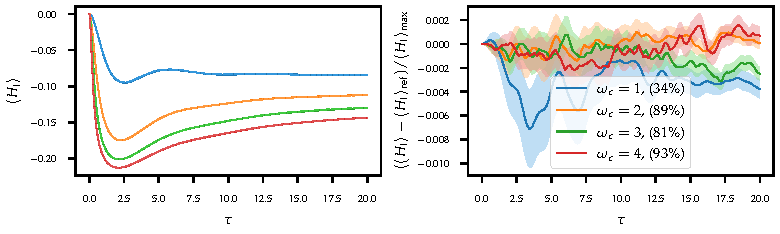
\includegraphics{figs/one_bath_syst/omega_interaction_consistency}
  \caption{\label{fig:omega_interaction_consistency}Interaction
    consistency plot for \cref{sec:one_bath_cutoff}, similar to
    \cref{fig:stocproc_systematics}.}
\end{figure}
\begin{figure}[H]
  \centering
  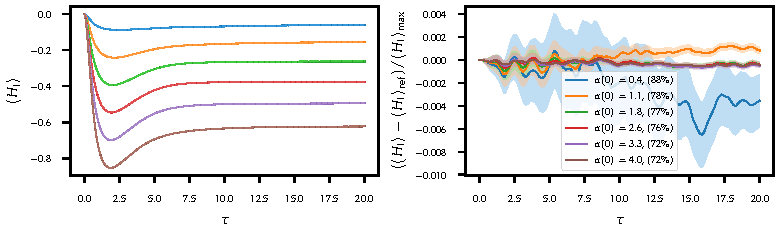
\includegraphics{figs/one_bath_syst/delta_interaction_consistency}
  \caption{\label{fig:delta_interaction_consistency}Interaction
    consistency plot for \cref{sec:one_bathcoup_strength}, similar to
    \cref{fig:stocproc_systematics}.}
\end{figure}

\subsection{Spectral Density Normalization}
\label{sec:spec_densities}
\begin{figure}[H]
  \centering
  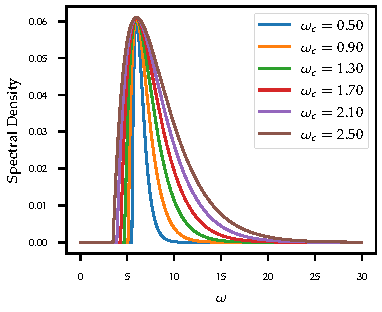
\includegraphics{figs/one_bath_mod/omega_sd_weak}
  \caption{\label{fig:omega_couplings_weak} Similar
    to \cref{fig:omega_couplings_and_energies} but for weaker coupling.}
\end{figure}


\subsection{More Plots for the Otto Cycle}
\label{sec:otto_plots}
\begin{figure}[H]
  \centering
  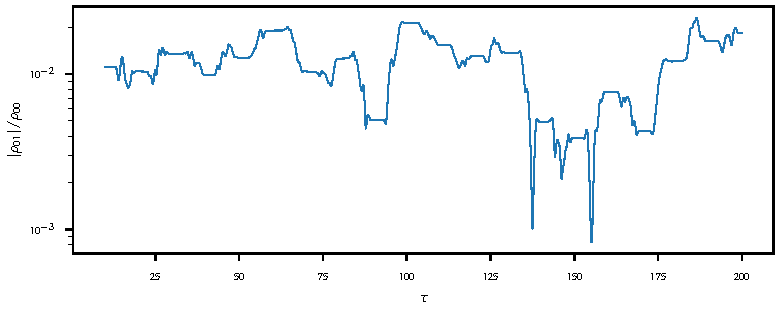
\includegraphics{figs/otto/coherences}
  \caption{\label{eq:otto_coherences} The coherences of the system
    state of the otto cycle in \cref{sec:otto}.}
\end{figure}
\begin{figure}[H]
  \centering
  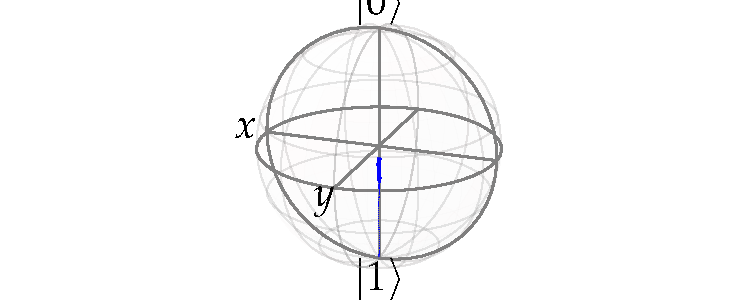
\includegraphics{figs/otto/bloch}
  \caption{\label{eq:otto_bloch} The system state of the model
    \cref{sec:otto} in the bloch sphere.}
\end{figure}

\section{Parameters}
\label{sec:plus_params}

\subsection{Modulation with a single Bath}
\label{sec:plus_mod_single}

\begin{table}
  \centering
  \begin{tabular}{lll}
    \hline
    $ω_c$              & $2$     & $2$    \\
    $α(0)$             & $0.7$   & $0.7$  \\
    $T$                & $5$     & $5$    \\
    $N$                & $10000$ & $2000$ \\
    $k_{\mathrm{max}}$ & $5$     & $5$    \\
    \hline
  \end{tabular}
  \caption{\label{tab:plus_friction}Additional parameters for
    \cref{fig:quant_frict}.}
\end{table}


\begin{table}
  \centering
  \begin{tabular}{lll}
    \hline
    $ω_c$              & $2$    & $2$    \\
    $α(0)$             & $0.7$  & $0.7$  \\
    $T$                & $5$    & $5$    \\
    $N$                & $1000$ & $1000$ \\
    $k_{\mathrm{max}}$ & $5$    & $5$    \\
    \hline
  \end{tabular}
  \caption{\label{tab:plus_system}Additional parameters for
    \cref{fig:quant_frict_sys_no_sys}.}
\end{table}

\begin{table}
  \centering
  \begin{tabular}{lllllll}
    \hline
    $ω_c$              & $0.50$     & $0.90$     & $1.30$     & $1.70$     & $2.10$     & $2.50$     \\
    $α(0)$             & $1.32$     & $1.42$     & $1.44$     & $1.33$     & $1.25$     & $1.37$     \\
    $T$                & $5.00$     & $5.00$     & $5.00$     & $5.00$     & $5.00$     & $5.00$     \\
    $N$                & $10000.00$ & $10000.00$ & $10000.00$ & $10000.00$ & $10000.00$ & $10000.00$ \\
    $k_{\mathrm{max}}$ & $5.00$     & $5.00$     & $5.00$     & $5.00$     & $5.00$     & $5.00$     \\
    BCF Terms          & $7.00$     & $7.00$     & $7.00$     & $7.00$     & $7.00$     & $7.00$     \\
    \hline
  \end{tabular}

  \caption{\label{tab:plus_omega}Additional parameters for the models in
     \cref{sec:extr_mem}.}
\end{table}


\begin{table}
  \centering
  \begin{tabular}{lllllll}
  \hline
   $ω_c$   & $ω_s$   & $α(0)$   & $T$    & $N$       & $k_{\mathrm{max}}$   & BCF Terms   \\
  \hline
   $1.00$  & $4.50$  & $0.78$   & $5.00$ & $1000.00$ & $7.00$               & $7.00$      \\
   $1.00$  & $4.62$  & $0.77$   & $5.00$ & $1000.00$ & $7.00$               & $7.00$      \\
   $1.00$  & $4.75$  & $0.76$   & $5.00$ & $1000.00$ & $7.00$               & $7.00$      \\
   $1.00$  & $4.88$  & $0.75$   & $5.00$ & $1000.00$ & $7.00$               & $7.00$      \\
   $1.00$  & $5.00$  & $0.74$   & $5.00$ & $1000.00$ & $7.00$               & $7.00$      \\
   $1.00$  & $5.12$  & $0.73$   & $5.00$ & $1000.00$ & $7.00$               & $7.00$      \\
   $1.00$  & $5.25$  & $0.72$   & $5.00$ & $1000.00$ & $7.00$               & $7.00$      \\
   $1.00$  & $5.38$  & $0.71$   & $5.00$ & $1000.00$ & $7.00$               & $7.00$      \\
   $1.00$  & $5.50$  & $0.70$   & $5.00$ & $1000.00$ & $7.00$               & $7.00$      \\
   $1.00$  & $4.50$  & $1.72$   & $5.00$ & $1000.00$ & $7.00$               & $7.00$      \\
   $1.00$  & $4.62$  & $1.70$   & $5.00$ & $1000.00$ & $7.00$               & $7.00$      \\
   $1.00$  & $4.75$  & $1.67$   & $5.00$ & $1000.00$ & $7.00$               & $7.00$      \\
   $1.00$  & $4.88$  & $1.65$   & $5.00$ & $1000.00$ & $7.00$               & $7.00$      \\
   $1.00$  & $5.00$  & $1.62$   & $5.00$ & $1000.00$ & $7.00$               & $7.00$      \\
   $1.00$  & $5.12$  & $1.60$   & $5.00$ & $1000.00$ & $7.00$               & $7.00$      \\
   $1.00$  & $5.25$  & $1.58$   & $5.00$ & $1000.00$ & $7.00$               & $7.00$      \\
   $1.00$  & $5.38$  & $1.56$   & $5.00$ & $1000.00$ & $7.00$               & $7.00$      \\
   $1.00$  & $5.50$  & $1.54$   & $5.00$ & $1000.00$ & $7.00$               & $7.00$      \\
  \hline
  \end{tabular}
  \caption{\label{tab:plus_tune}Additional parameters for the models in
     \cref{sec:modcoup_reso}.}
\end{table}
